\documentclass[a4paper,10pt]{article}
\usepackage[utf8]{inputenc}
\usepackage{graphicx}
\DeclareGraphicsExtensions{.eps,.mps,.pdf,.jpg,.png}
\title{Assignment for QRM}
\author{Lu Lin}

\begin{document}

\maketitle




\section{Introduction}

\paragraph{This article is to show the evidence of the geography divergence on the development of crowdfunding industry and reveal several important factors may affect the successful rate of crowdfunding. Firstly, the crowdfunding can be seen as an alternative way to fund money from public, particular for start-up or SMEs, compared with traditional way, such as IPO or Bank loan. The main investors in the crowdfunding industry are the crowd. Thus, the way to attract the crowd’s attentions or draw crowd’s interesting points and encourage them to join this finance game is the main aim. }
\paragraph{In this article, the crowdfunding data comes from the one of largest crowdfunding platform: Kickstarter.com, and the state-based data comes from the U.S. Bureau of Labour Statistics. All data are the 2010 year data. And all data can be found in the Appendix. By analysing the secondary public data, some graphical evidence and empirical findings demonstrate the ****}


\section{Method and Analysis}



\subsection{Geography Information: Region difference on the crowdfunding successful rate and number of launched project}


\paragraph{The Figure \ref{Boxplots_for_Count_and_SR} shows a group of Count of project boxplot(left), Log Count of project boxplot (middle) and Successful rate boxplot(right) based on different region. In the Count of project boxplot(left) and Log Count of project boxplot(middle), excluding the outliers or abnormal value, the median of count of launched project grouped by region do not show significant different from others. Although, there is no significant different in graphical plot. Obviously, the minimum and lower whisker of Northeast seem be higher than those of others, and maximum and upper whisker of it also are higher than others. This graphical information suggests me that the people from Northeast seem be more likely to set up a crowdfunding project. However, in the Successful rate boxplot, the successful rate of Northeast looks like have a strong different from other three. The five numbers (minimum, lower whisker, median, upper whisker and maximum) in the successful rate from northeast are all significant higher from that of others. It implies that the project which is launched in northeast seem be more popular and easier to fund money, compared with other regions.}

\begin{figure}
	\centering
	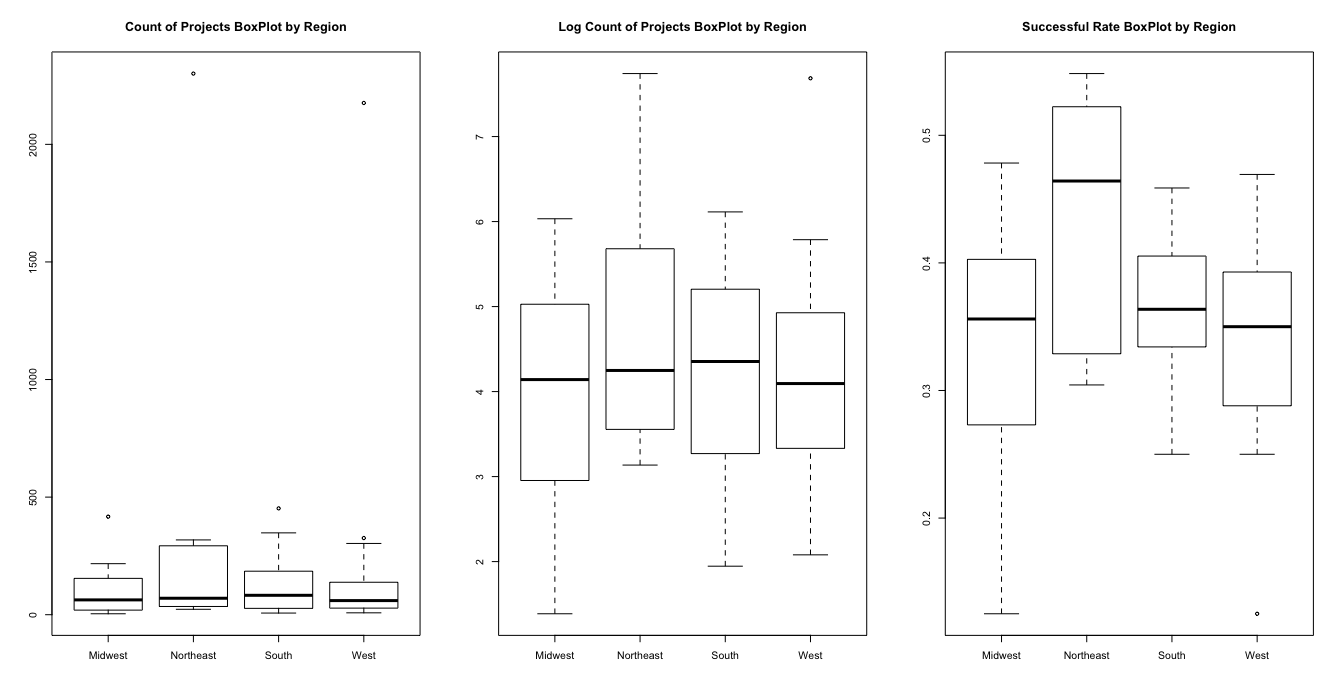
\includegraphics[width = \textwidth]{comparative_boxplots_for_Count_and_SR}
	\caption[Comparative boxplots of Count of projects(left), Log Count of project(middle) and Successful rate(right) by Region]{Comparative boxplots of Count of projects(left), Log Count of project(middle) and Successful rate(right) by Region}
	\label{Boxplots_for_Count_and_SR}
\end{figure}
\paragraph{}
Furthermore, on skewness, the count of project in Northeast has a positive skewness and rest seem be zero skewness. The successful rate of Northeast show a slightly negative skewness and the successful rate of Mideast demonstrate a negative skewness. The rest distribution do not show a particular skew.Hence, the Q-Q Norm should be used to show the distribution of the variables. From Figure \ref{Count and SR qqnorm}, there seem be not strictly following the normal distribution. And the all of Successful Rate and Count of projects categoried by Region show the positive kurtosis. However, as the figure shown, the sample size of each plot is less 30.
\begin{figure}
	\centering
	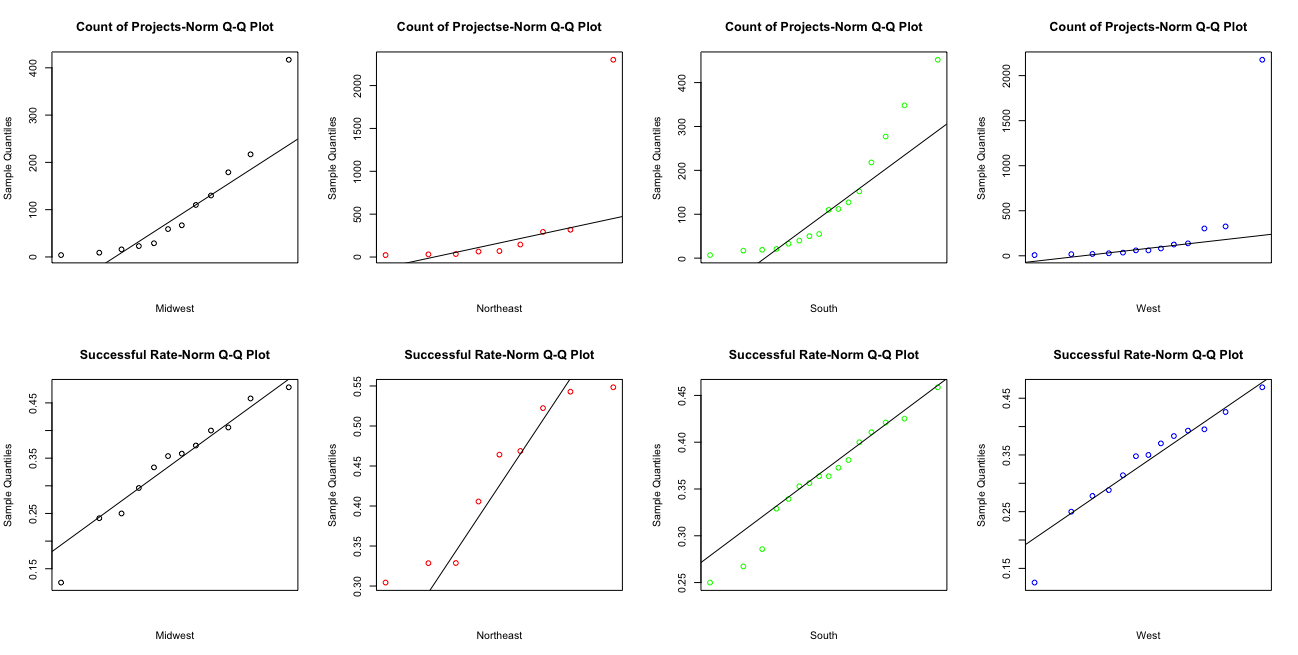
\includegraphics[width = 1\textwidth]{count_and_SR_qqnorm}
	\caption{Q-Q norm of Count of Projects and Successful rate by Region}
	\label{Count and SR qqnorm}
\end{figure}










\paragraph{}
Overall, from those graphical evidence, there are the Regional difference on the crowdfunding successful rate and count of projects. The development of crowdfunding and the successful rate of crowdfunding project in Northeast seem own a significant different from other regions. Here, there is necessary to use empirical (parametric) test on this finding. Before doing test, here gives the Null hypothesis and alternation hypothesis:
\paragraph{}
H0: The Northeast has no different crowdfunding successful rate than other regions.
	\\Ha: The Northeast has no different crowdfunding successful rate than other regions.
\paragraph{}Because of small and Unequal sample size, I use bootstrap method to resample each group and use resampled group data to test hypothesis. From the table 1, all p-value are smaller than 2.2e-16, which suggest me to reject my Null Hypothesis. Meanwhile, all t-value are positive number, which show that  the project created in the northeast own a significantly higher successful rate than rest of regions.

\subsection{Factors: Gini Coefficient and Advanced Education}

\subsubsection{Successful Rate-Gini Coefficient}
\subsubsection{Successful Rate-Advanced Education}

\subsubsection{Interrelation on GiniCoeff and Advanced Education
}
\medskip

\section{Conclusion}

\section{Appendix}

\end{document}